% Diese Zeile bitte -nicht- aendern.
\documentclass[course=erap]{aspdoc}

%%%%%%%%%%%%%%%%%%%%%%%%%%%%%%%%%
\newcommand{\theGroup}{110}
\newcommand{\theNumber}{A201}
\author{Simon Bußmann \and Nico Lintner \and Manuel Walter Mußbacher}
\date{Sommersemester 2023}
%%%%%%%%%%%%%%%%%%%%%%%%%%%%%%%%%

% Diese Zeile bitte -nicht- aendern.
\title{Gruppe \theGroup{} -- Abgabe zu Aufgabe \theNumber}

\usepackage{caption}
\usepackage{subcaption}

\begin{document}
\maketitle

\section{Einleitung}

In diesem Projekt haben wir uns damit beschäftigt, den Sobel-Filter Algorithmus zu implementieren.
Dieser Algorithmus wird verwendet, um Kanten in Bildern zu erkennen.
Dabei werden die Pixel eines Bildes mit zwei Matritzen, sogenannte Filter, verrechnet.
Die aus dieser Verrechnung resultierenden Werte werden dann in einem neuen Bild gespeichert.
\begin{figure}[H]
    \begin{subfigure}{.5\columnwidth}
        \centering
        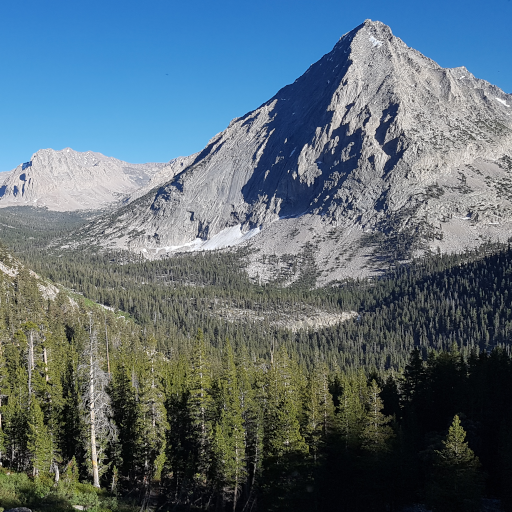
\includegraphics[width=\columnwidth]{graphics/johnmuirtrail.png}
        \caption{Input-Bild}
        \label{fig:input-bild}
    \end{subfigure}
    \begin{subfigure}{.5\columnwidth}
        \centering
        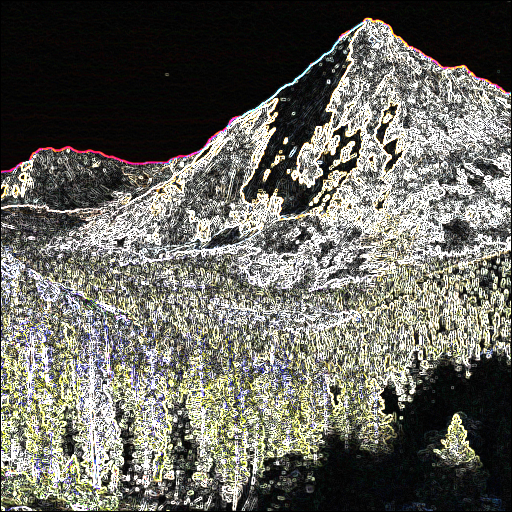
\includegraphics[width=\columnwidth]{graphics/johnmuirtrail_sobel.png}
        \caption{Output-Bild}
        \label{fig:output-bild}
    \end{subfigure}
\end{figure}

In Abbildung \ref{fig:input-bild} und \ref{fig:output-bild} ist ein Beispiel für die Anwendung des Sobel-Filters zu sehen.

\section{Lösungsansatz}

Unser gewählter Lösungsansatz besteht aus drei verschiedenen Versionen.
In der ersten Version haben wir den Sobel-Filter nach seiner mathematischen Definition implementiert.
Zusätzlich dient und die erste Version als Vergleichsimplementierung.
Die zweite und dritte Version sind jeweils eine Optimierung der ersten Version.
In der zweiten Version haben wir die den Algorithmus mit Hilfe von SIMD-Instruktionen implementiert und in der dritten die SIMD Implementierung mit Threading kombiniert.
Alle Implementierungen arbeiten mit 24-Bit BMP Bildern. Ein Pixel besteht dabei aus drei Bytes, die die Farbwerte Rot, Grün und Blau repräsentieren.

\subsection{Vergleichsimplementierung}
Die Vergleichsimplementierung ist eine naive Implementierung des Sobel-Filter Algorithmus.
Dabei werden die beiden Filtermatritzen $M^{v}$ und $M^{h}$ mit jedem Pixel des Bildes verrechnet.
\begin{equation}
    M^{v} :
    \begin{bmatrix}
        1 & 0 & -1 \\
        2 & 0 & -2 \\
        1 & 0 & -1
    \end{bmatrix}
    M^{h} :
    \begin{bmatrix}
        1 & 2 & 1 \\
        0 & 0 & 0 \\
        -1 & -2 & -1
    \end{bmatrix}
\end{equation}
\begin{equation}
    A^{h} = M^{h} * Image
\end{equation}
\begin{equation}
    A^{v} = M^{v} * Image
\end{equation} \\
Jeder Pixel besteht aus drei Bytes, die die Farbwerte Rot, Grün und Blau repräsentieren.
Deswegen wird das Bild B in drei Farbkanäle F aufgeteilt.
Um einen Pixel mit den Filtermatritzen zu verrechnen, werden die Werte der Filtermatrix mit den Werten der umliegenden Pixel multipliziert und anschließend aufsummiert.
\begin{equation}
    A_(x,y)^{v,F} = \sum_{i=-1}^{1} \sum_{j=-1}^{1} M^{v}_{i,j} * B_{(x+i,y+j)}^{F}
\end{equation}
\begin{equation}
    A_(x,y)^{h,F} = \sum_{i=-1}^{1} \sum_{j=-1}^{1} M^{h}_{i,j} * B_{(x+i,y+j)}^{F}
\end{equation}
Um nun den Sobelwert eines Pixels zu berechnen wird der Betrag der horizontalen und vertikalen Sobelwerte berechnet.
\begin{equation}
    O^{F}_{x,y} = \left | A^{v,F}_{x,y} \right | + \left | A^{h,F}_{x,y} \right |
    \label{eq:betrag}
\end{equation}
Pixel, die sich am Rand des Bildes befinden, können nicht mit allen Werten der Filtermatritzen verrechnet werden.
Der Fall wird behandelt, indem die Sobelwerte dieser Pixel als schwarz angenommen werden. Hierdurch entsteht ein schwarzer Rand um das Bild.
\\\\
Normalerweise wird im letzten Schritt der Endgültige Sobel Wert mit der Wurzel der Summe der Quadrate berechnet.
\begin{equation}
    O^{F}_{x,y} = \sqrt{(A^{v,F}_{x,y})^2 + (A^{h,F}_{x,y})^2}
    \label{eq:wurzel}
\end{equation}
\begin{figure}[H]
    \begin{subfigure}{.5\columnwidth}
        \centering
        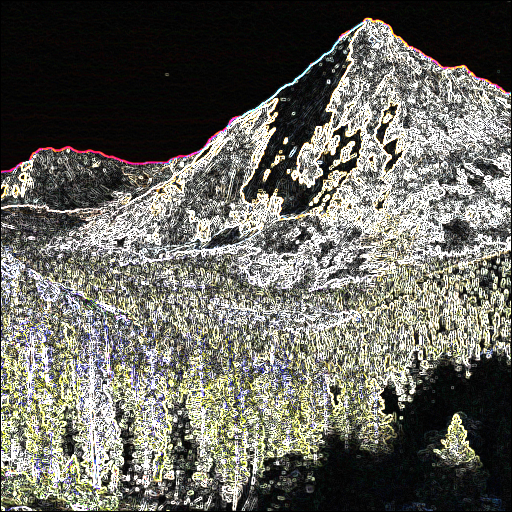
\includegraphics[width=\columnwidth]{graphics/johnmuirtrail_sobel.png}
        \caption{Abs Version \ref{eq:betrag}}
        \label{fig:abs-bild}
    \end{subfigure}
        \begin{subfigure}{.5\columnwidth}
        \centering
        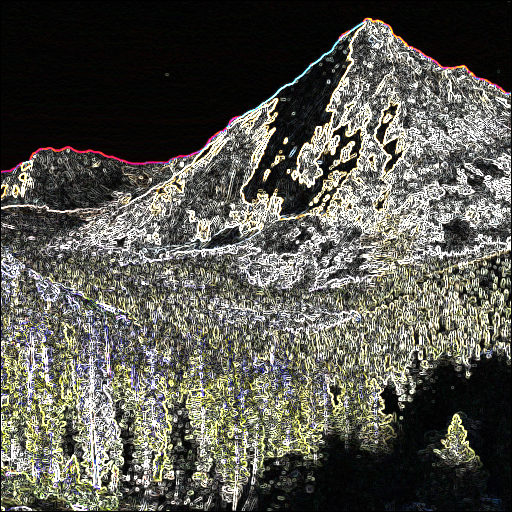
\includegraphics[width=\columnwidth]{graphics/sqrt_sobel.png}
        \caption{Sqrt Version \ref{eq:wurzel}}
        \label{fig:sqrt-bild}
    \end{subfigure}
\end{figure}
Zwischen {\ref{fig:abs-bild}} und {\ref{fig:sqrt-bild}} besteht nur ein kleiner Unterschied in der Helligkeit des Bildes, was für Kantenerkennung nicht relevant ist.
Da keine SIMD-Instruktion zur Berechnung der Wurzel eines 8 bzw. 16 Bit Integers existiert und diese Version als Vergleichsimplementierung genutzt werden soll, haben wir uns für die Variante {\ref{eq:betrag}} entschieden.
\subsection{SIMD Implementierung}
Die SIMD Implementierung basiert auf der Vergleichsimplementierung, benutzt zur Berechnung jedoch SIMD Instruktionen.
Ein großes Problem, bei der Arbeit mit 8-Bit-Ganzzahlen ist der kleine Wertebereich.
Da die Werte der einzelnen Farbchannel der Pixel als 8 Bit Integer gespeichert werden, kann es folglich bei der Faltungsoperation schnell zu einem Überlauf kommen.
Der naive Lösungsansatz, um dem entgegen zu wirken, ist das Input-Bild einfach um 75\% zu verdunkeln.
Durch die Verdunkelung wird der Überlauf zwar verhindert, das Output Bild ist jedoch auch (wesentlich) dunkler {\ref{fig:dark}}, wodurch die erkannten Kanten signifikant dunkler werden.
\begin{figure}[H]
    \begin{subfigure}{.5\columnwidth}
        \centering
        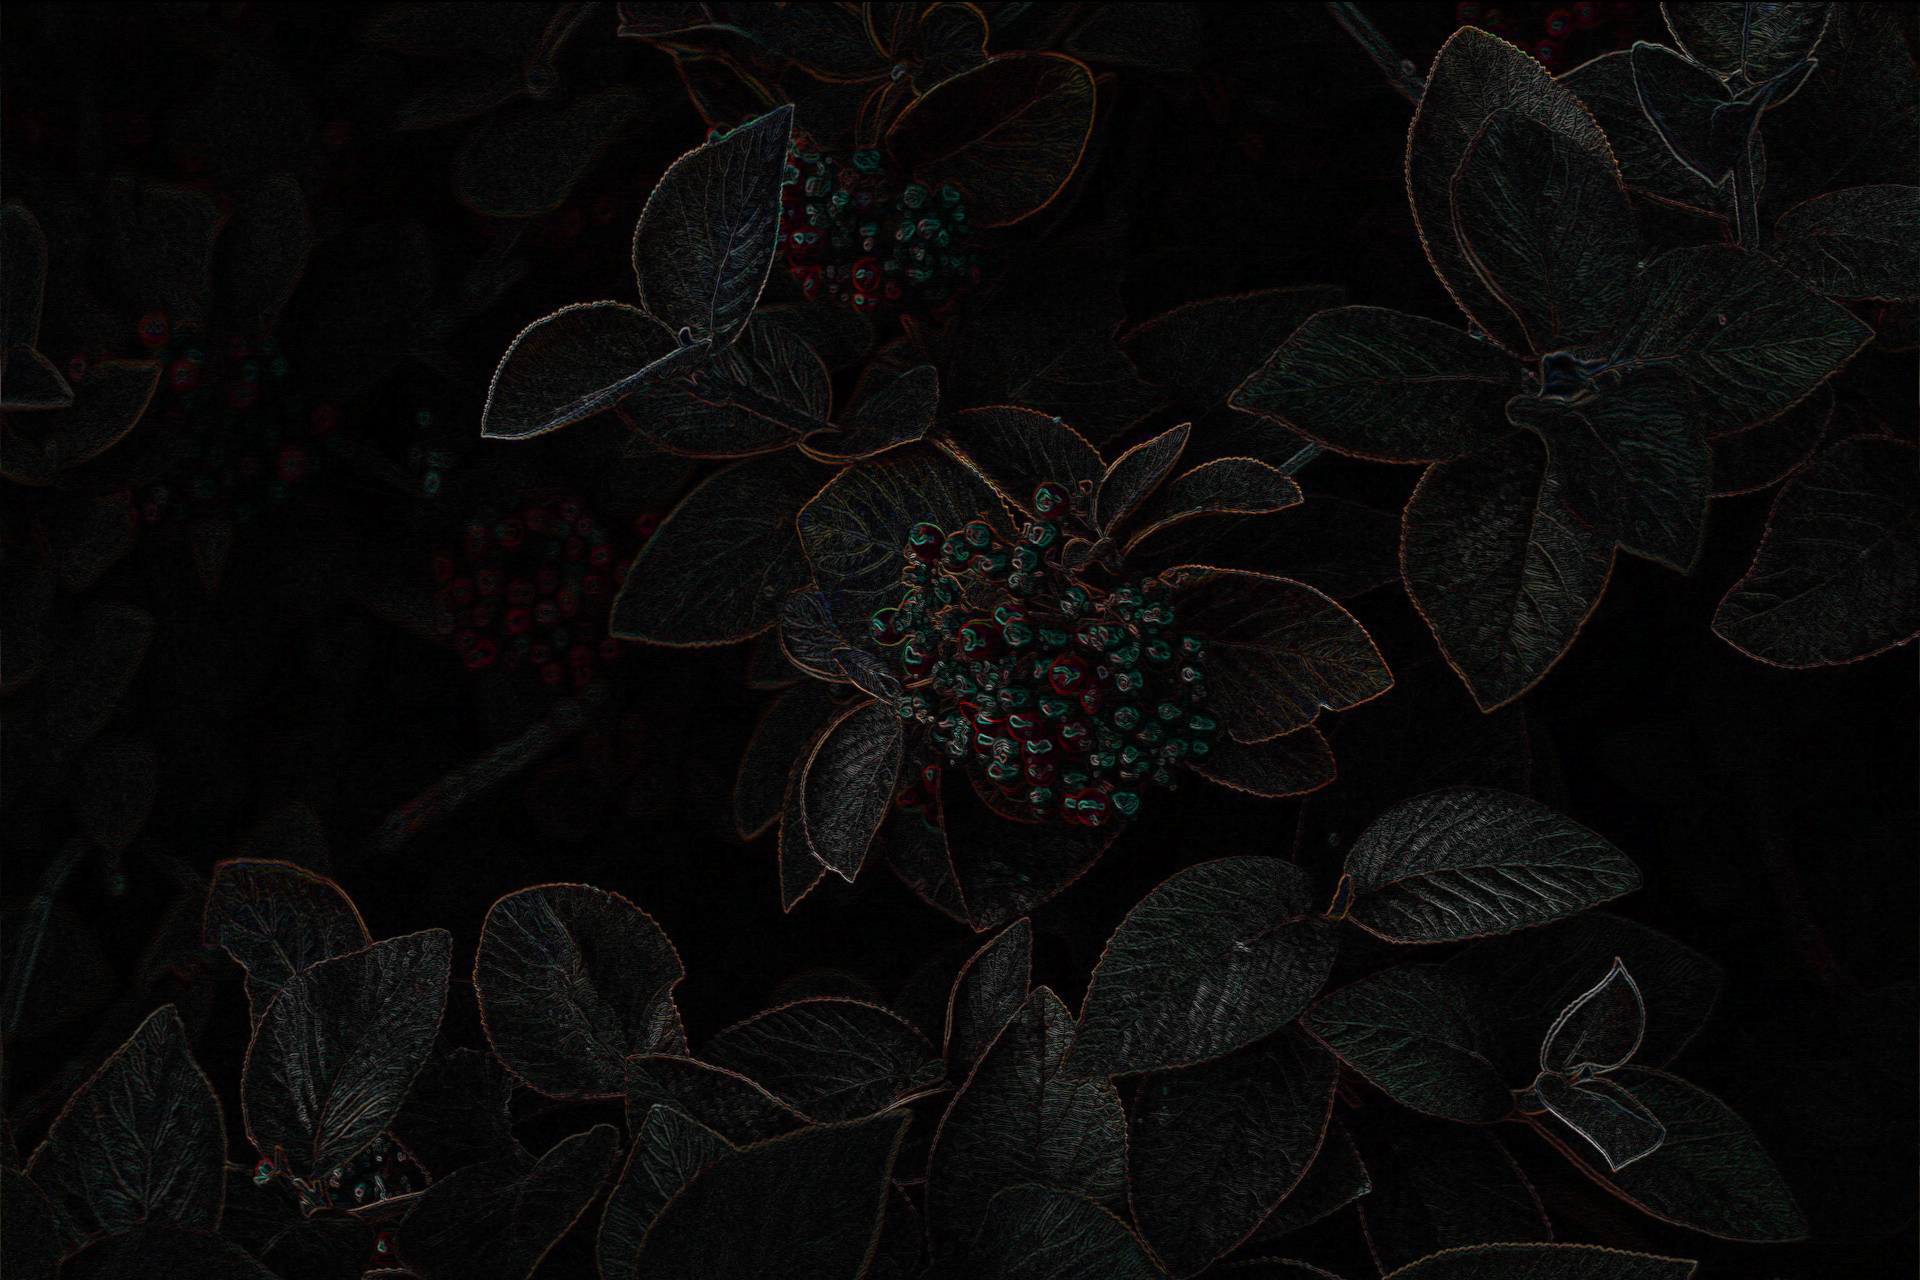
\includegraphics[width=\columnwidth]{graphics/dark.png}
        \caption{Erste SIMD Version}
        \label{fig:dark}
    \end{subfigure}
    \begin{subfigure}{.5\columnwidth}
        \centering
        \includegraphics[width=\columnwidth]{graphics/correct.png}
        \caption{Vergleichsimplementierung}
        \label{fig:correct}
    \end{subfigure}
\end{figure}
Um trotz Vektorinstruktionen und sehr kleinen Wertebereichen ein Ergebnis zu erzielen,
das - bis auf den linken und rechten Rand - exakt der Vergleichsimplementierung entspricht,
werden die Daten aus einem 16-Byte-Speicherbereich so in zwei Vektoren geladen, dass während der Berechnung je 8 Byte
als 16-Bit-Integer interpretiert werden können.
Dabei werden insgesamt 16 xmm Register benutzt, um jeweils die Sobel Werte für 16 Farbchannel zu berechnen.
Das funktioniert so, dass ein 16 Byte-Speicherbereich gelesen wird und anschließend das jeweils höherwertige Byte eines jeden
16-Bit-Integers in diesem Vektor mit einer Bitmaske genullt wird. Das geschieht analog mit den 16-Byte an der um einen Byte höheren Speicheradresse.
Für jeden der 16 Farbchannel, die mit einem Schleifendurchlauf berechnet werden können, werden so die acht umliegenden
Farbchannel geladen. Dadurch lassen sich die Farbwerte für 16 Byte gleichzeitig berechnen. Durch den dadurch entstehenden Overhead
ist dieser Lösungsansatz zwar ca. nur halb so schnell, wie der naive SIMD-Ansatz, erzeugt jedoch wesentlich
akkuratere Ergebnisse, weshalb das Programm auch diesen Ansatz implementiert. In Relation zur Vergleichsimplementierung erzielt dieser
Ansatz in etwa einen Speedup von x10.

\subsection{SIMD-Implementierung mit Threading}
Die SIMD-Implementierung mit Threading basiert auf der SIMD-Implementierung mit der Besonderheit, dass das Bild in Abschnitte eingeteilt werden, die jeweils von einem eigenen Thread bearbeitet werden.
Um diese Abschnitte zu erzeugen, wird das Bild in horizontale Streifen geschnitten. Die Anzahl dieser Streifen hängt davon ab, wie viele Zeilen pro Thread berechnet werden sollen.
Das horizontale Zerteilen des Bildes hat den Vorteil, dass der Cache besser genutzt wird, als zum Beispiel beim Aufteilen in Quadranten, weil die Daten hintereinander Zeile für Zeile im Speicher liegen.
Desweiteren besteht der Vorteil, fortlaufende Indizes bei der Berechnung nutzen zu können und nicht, wie zum Beispiel bei einer Aufteilung in Quadranten, diese Indizes aufwendig berechenen zu müssen.

\section{Genauigkeit}
Wir haben uns dafür entschieden, die Genauigkeit unseres Lösungsansatzes zu analysieren, da es bei Kantenerkennung keine fest definierte "source of truth", wie zum Beispiel bei einer pur mathematischen Operation, gibt.
Öffentlich existierende Sobel Filter Implementierungen wie zum Beispiel die von OpenCV
\section{Performanzanalyse}

TODO: Geben Sie hier die Performanz Ihres Lösungsansatzes ein.

\section{Zusammenfassung und Ausblick}

TODO: Geben Sie hier eine kurze Zusammenfassung und einen Ausblick ein.

% TODO: Fuegen Sie Ihre Quellen der Datei Ausarbeitung.bib hinzu
% Referenzieren Sie diese dann mit \cite{}.
% Beispiel: CR2 ist ein Register der x86-Architektur~\cite{intel2017man}.
\bibliographystyle{plain}
\bibliography{Ausarbeitung}

\end{document}
